\documentclass[varwidth=true, border=2pt]{standalone}

\usepackage{pgfplots}
\usepackage{tikz}

\begin{document}
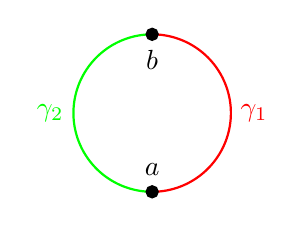
\begin{tikzpicture}
    \tikzstyle{point}=[circle,thick,draw=black,fill=black,inner sep=0pt,minimum width=4pt,minimum height=4pt]
    \draw [red,  thick,domain=90:-90,  samples=100] plot ({cos(\x)}, {sin(\x)});
    \draw [green,thick,domain=-90:-270,samples=100] plot ({cos(\x)}, {sin(\x)});
    \node (a)[point,label=90:$a$] at (0,-1cm) {};
    \node (b)[point,label=-90:$b$] at (0, 1cm) {};

    \node at (1,0) [anchor=180, red] {$\gamma_1$};
    \node at (-1,0) [anchor=0, green] {$\gamma_2$};

\end{tikzpicture}
\end{document}
